\section{Properties of universal packings}
\noindent Let us examine the properties of Hoffman packings and universal packings.
In \cite[p. 1]{Spiridonov_2003} Spiridonov stipulates that the structure of a three-dimensional packing of a dimension tuple satisfying Hoffman's inequality must be rigid and notes that ``this is probably not necessary; however, it seems tricky to show that no loose packings exist''. We will not attempt to prove this, but we will provide an intuitive argument as to why it is well-founded to claim that a packing of a dimension tuple satisfying Hoffman's inequality and consisting solely of hyperrectangles is rigid.

Suppose $P$ is a Hoffman packing of a dimension tuple $d$ satisfying Hoffman's inequality and let $(B, C)$ be the packing of $d$ produced by $P$. We would like to argue that any rearrangements of this packing is identical to itself. We do so by eliminating the possibility of moving any of the hyperrectangles in $B$. By Hoffman's grid theorem \labelcref{thm:grid-theorem} each of the $n^n$ hyperrectangles contains precisely one grid point. Pick some grid point $c$ with coordinates $p$ and let $R_p$ be the hyperrectangle in $B$ associated with $p$, i.e.\ containing $c$. We begin by ruling out any translations. Consider some dimension $k$ in $\curly{1, 2, \dotsc, n}$ and observe that the hyperrectangles associated with the grid points on the line through $p$ along the $k$'th dimension all intersect the line
\[
L_k = V_1 \times V_2 \times \dotsb \times V_n,
\]
where $V_k = \R$ and $V_i = \curly{c_i}$ for all $i \neq k$. Thus, along all dimensions $R_p$ is wedged between two hyperrectangles (or the surrounding hypercube) due to Hoffman's line theorem \labelcref{thm:line-theorem}, see \cref{fig:wedged-with-line-fixed}. Intuitively, this is enough to eliminate any continuous translation of the hyperrectangle, since the slightest translation along any dimension will result in the hyperrectangle overlapping with some adjacent hyperrectangle. What about rotations? In \cref{fig:wedged-and-loose} it is illustrated how being wedged between two hyperrectangles along all dimensions is not enough to prevent rotations. However, if along all dimensions there is a line running through the hyperrectangle and the adjacent hyperrectangles along that dimension, then the hyperrectangle can not be continuously rotated without overlapping with an adjacent hyperrectangle, see \cref{fig:wedged-with-line-fixed}.

\begin{figure}[ht]
    \centering
    \begin{subfigure}[b]{0.45\textwidth}
        \centering
            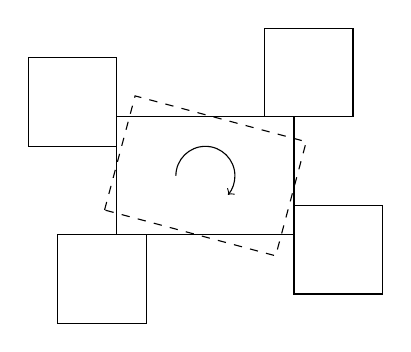
\begin{tikzpicture}[scale=0.75]
                \draw[] (0, 0) rectangle (3, 2);
                \draw[->] (1, 1) arc (180:-40:0.5);
                \draw[] (-1, -1.5) rectangle (0.5, 0);
                \draw[] (-1.5, 1.5) rectangle (0, 3);
                \draw[] (3, -1) rectangle (4.5, 0.5);
                \draw[] (2.5, 2) rectangle (4, 3.5);
                \draw[dashed, rotate around={-15:(1.5, 1)}] (0, 0) rectangle (3, 2);
            \end{tikzpicture}
        \caption{Rectangle which can not be translated, since it is wedged between two rectangles along each dimension. Observe however, that it \textit{can} be rotated.}
        \label{fig:wedged-and-loose}
    \end{subfigure}
    ~
    \begin{subfigure}[b]{0.45\textwidth}
        \centering
            \begin{tikzpicture}[scale=0.75]
                \draw[] (0, 0) rectangle (3, 2);
                \draw[] (0.5, -1.5) rectangle (2, 0);
                \draw[] (-1.5, 0.5) rectangle (0, 2);
                \draw[] (3, 0.25) rectangle (4.5, 1.75);
                \draw[] (1.5, 2) rectangle (3, 3.5);
                \draw[dashed] (-1.75, 0.75) -- (4.75, 0.75);
                \draw[dashed] (1.75, -1.75) -- (1.75, 3.75);

                \node at (0, 2) [anchor=north west] {$R_p$};
                \filldraw (1.75, 0.75) circle (2pt) node[anchor=north west] {$c$};
            \end{tikzpicture}
        \caption{Rectangle which can not be translated or rotated, since along each dimension there is a line passing through it and the adjacent rectangles.}
        \label{fig:wedged-with-line-fixed}
    \end{subfigure}
    \caption{Examples illustrating what is necessary to ensure that a hyperrectangle can not be moved.}
\end{figure}

\noindent Lastly, we consider the feasibility of moving multiple hyperrectangles simultaneously. Then in particular we move some specific hyperrectangle $R$. But moving $R$ forces us to also move some adjacent hyperrectangle to prevent overlap and this causes a chain reaction resulting in one of the hyperrectangles pricking a hole in the surrounding hypercube $C$ and thus no longer constituting a packing. Hence, without further ado we will state the following proposition.

\begin{proposition}\label[proposition]{prop:hoffman-packing-rigid}
Suppose $d$ is a dimension tuple satisfying Hoffman's inequality and suppose $(B, C)$ is a packing of $d$ consisting solely of hyperrectangles. Then $(B, C)$ is a rigid packing.
\end{proposition}

\noindent The following result limits the number of universal packings being equivalent.

\begin{lemma}\label[lemma]{lemma:finding-tuples}
There exists a strictly increasing sequence of $n$ positive real numbers $x_1 < x_2 < \dotsb < x_n$ such that $\paren{x_1, x_2, \dotsc, x_n}$ satisfies Hoffman's inequality and such that the only way to add an arbitrary number of these sequence elements up to $x_1 + x_2 + \dotsb + x_n$ is to add precisely one of each.
\end{lemma}
\begin{proof}
The case $n = 1$ is trivial, so suppose $n \geq 2$. Define a sequence of $n$ positive real numbers by $x_i = 1 + n^{-(n-i+1)}$ for $i = 1, 2, \dotsc, n$. Note that this sequence is strictly increasing since
\[
x_{i+1} - x_i
= n^{-(n-i)} - n^{-(n-i+1)}
= n^{-(n-i)}(1 - 1/n) > 0
\]
for all suitable $i$. We now represent each sequence element in base-$n$. Then the fractional part of $x_i$ consists of $n-i$ zeros followed by a one for all $i = 1, 2, \dotsc, n$, i.e.\ $x_n = 1.1_n$, $x_{n-1} = 1.01_n$ and so on. We denote the sum consisting of precisely one of each sequence element by $s$ and we see that
\[
s = x_1 + x_2 + \dotsb + x_n = 10.\overbrace{11 \dotso 1}^{\text{$n$ ones}}\!{}_n.
\]
Notice that any sum of sequence elements with more than $n$ terms will be strictly greater than $s$, since the integer part of the sum would be at least $11_n$. In particular, the sequence satisfies Hoffman's inequality.

Suppose there exists a sum of sequence elements with $n$ or fewer terms such that they add up to $s$. Consider the base-$n$ representation of this sum. Precisely one of the terms must be $x_1$, since this is the only way to obtain a one at the $n$'th position of the fractional part of the sum. Similarly, we can now conclude that precisely one term must be $x_2$ and using induction the sum must have $n$ terms with precisely one $x_i$ term for each $i = 1, 2, \dotsc, n$.
\end{proof}

\begin{lemma}\label[lemma]{lemma:distinct-hoffman-packings-different}
Suppose $d$ is a dimension tuple with distinct elements. If $P_1$ and $P_2$ are Hoffman packings of $d$ producing the same packing, then $P_1 = P_2$.
\end{lemma}
\begin{proof}
Let $(B, C)$ be the packing produced by $P_1$ and $P_2$. Suppose $p$ is a grid point coordinate in $G_n$. We would like to show that $P_1(p) = P_2(p)$. Consider the dimension tuple $r$ of the hyperrectangle $R_p$ in $B$ associated with $p$. Since the elements of $d$ are distinct there is only one permutation $\sigma$ in $S_n$ such that $(d_{\sigma(1)}, d_{\sigma(2)}, \dotsc, d_{\sigma(n)}) = r$, whereby $P_1(p) = \sigma = P_2(p)$.
\end{proof}

\begin{proposition}\label[proposition]{prop:universal-symmetries}
A unique universal packing contains at most $n! \cdot 2^n$ universal packings.
\end{proposition}
\begin{proof}
Suppose $\Omega$ is a unique universal packing. Let $d$ be the dimension tuple consisting of the sequence given by \cref{lemma:finding-tuples}. Then all of the Hoffman packings in $\Omega$ produce packings of $d$, which are equivalent. However, none of them are identical due to \cref{lemma:distinct-hoffman-packings-different}. By \cref{prop:hoffman-packing-rigid} these packings are rigid, so there are at most $n! \cdot 2^n$ of them, namely their symmetries. Thus, there are at most $n! \cdot 2^n$ Hoffman packings in $\Omega$.
\end{proof}

\subsection{Verifying a Hoffman packing}
When assessing whether a map $P \colon G_n \to S_n$ is in fact a universal packing we need to show that it is a Hoffman packing of any dimension tuple $d$ satisfying Hoffman's inequality. Therefore we seek a clever way of ensuring that the pseudo-packing $(B, C)$ produced by $P$ is in fact a packing of $d$. Hence, we need to make sure that all of the hyperrectangles in $B$ are contained in the surrounding hypercube $C$ and that the hyperrectangles in $B$ are pairwise non-overlapping. Let us begin with a criterion which ensures that the hyperrectangles are contained in the surrounding hypercube.

\begin{criterion}[Line criterion]\label[criterion]{criterion:line-criterion}\index{Criterion!line}
Suppose $P\colon G_n \to S_n$. Let $d = \paren{x_1, x_2, \dotsc, x_n}$ be a dimension tuple with distinct elements and consider the pseudo-packing $(B, C)$ of $d$ produced by $P$. A grid line along some dimension $k \in \curly{1, 2, \dotsc, n}$ is a \textit{unique line}\index{Grid line!unique} if for all $i = 1, 2, \dotsc, n$ there is precisely one grid point $p$ on the grid line where the associated hyperrectangle has an extent of $x_i$ along the $k$'th dimension, i.e.\ $P(p)(k) = i$. If all grid lines are unique lines, then $P$ satisfies the \textit{Line criterion}.
\end{criterion}

\begin{remark}
The Line criterion \labelcref{criterion:line-criterion} is inspired by Hoffman, who introduced it in the three-dimensional case \cite[p. 220]{Hoffman1981}. However, Hoffman's way of justifying it does not scale easily to higher dimensions. However, as we will see below, the notion of a universal packing does in fact allow us to require it in higher dimensions.
\end{remark}

\noindent It follows from the next result that the Line criterion \labelcref{criterion:line-criterion} will guarantee the hyperrectangles to be contained in the surrounding hypercube.

\begin{proposition}\label[proposition]{prop:under-stuffed-contains-rects}
Suppose $P \colon G_n \to S_n$. Let $d$ be a dimension tuple and let $s$ be its sum. Let $(B, C)$ be the pseudo-packing of $d$ produced by $P$. If the stuffing on each grid line is no bigger than $s$, then all of the hyperrectangles in $B$ are contained in the surrounding hypercube $C$.
\end{proposition}
\begin{proof}
Recall that $C = (0, s)^n$. Suppose $p$ is a grid point coordinate in $G_n$ and let $R_p$ denote the associated hyperrectangle in $B$. Using the notation from \cref{def:hoffman-packing}, we can write $R_p$ as the Cartesian product
\[
R_p = \prod_{i = 1}^n (a(p)_i, b(p)_i)
= (a(p)_1, b(p)_1) \times (a(p)_2, b(p)_2) \times \dotsb \times (a(p)_n, b(p)_n).
\]
Let $v$ be an element in $R_p$ and note that $a(p)_i < v_i < b(p)_i$ for all $i = 1, 2, \dotsc, n$. In order to show that $v$ lies in $C$, we need to show that $0 < v_i < s$ for all $i = 1, 2, \dotsc, n$.

Take some $i$ in $\curly{1, 2, \dotsc, n}$. By examining the definition of the $i$'th element of the anchor-point $a(p)$ in \cref{def:hoffman-packing}, we observe that $a(p)_i$ is a sum of non-negative real numbers. Hence, $a(p)_i$ is non-negative itself, whereby $0 \leq a(p)_i < v$. Next, consider $b(p)_i = a(p)_i + w(p)_i$, which can be recursively unwrapped into
\[
b(p)_i = \sum_{k = 1}^{p_i} w(L(p, i, k))_i \leq \sum_{k = 1}^{n} w(L(p, i, k))_i \leq s,
\]
since the stuffing on the grid line running through $p$ along dimension $i$ is no bigger than $s$. Then $v_i < b(p)_i \leq s$, so $v$ is in $C$. Thus, $R_p$ is contained in $C$ as desired.
\end{proof}

\noindent Next, we show that restricting the search for universal packings to maps $P\colon G_n \to S_n$ satisfying the Line criterion \labelcref{criterion:line-criterion} does not overlook any universal packings.

\begin{proposition}\label[proposition]{prop:universal-packing-has-unique-lines}
Suppose $P$ is a universal packing. Then $P$ satisfies the Line criterion \labelcref{criterion:line-criterion}.
\end{proposition}
\begin{proof}
Let $d = \paren{x_1, x_2, \dotsc, x_n}$ be the dimension tuple consisting of the sequence given by \cref{lemma:finding-tuples} and let $s$ denote its sum. Observe that the elements of $d$ are distinct, since it is strictly increasing. Let $(B, C)$ be the packing of $d$ produced by $P$. Take some grid line along some dimension $k \in \curly{1, 2, \dotsc, n}$. We would like to show that this is a unique line. Since $d$ satisfies Hoffman's inequality this grid line is completely stuffed by Hoffman's line theorem \labelcref{thm:line-theorem}. Recall that by \cref{lemma:finding-tuples} the only way to add the elements of $d$ up to $s$ is to use precisely one of each. There are $n$ grid points on the grid line, so for each $i = 1, 2, \dotsc, n$ there must be precisely one grid point $p_i$ on the grid line for which the associated hyperrectangle has an extent of $x_i$ along the $k$'th dimension, i.e.\ $P(p_i)(k) = i$. Hence, the grid line is a unique line, whereby $P$ satisfies the Line criterion \labelcref{criterion:line-criterion}.
\end{proof}

\noindent It remains to ensure that the hyperrectangles are pairwise non-overlapping. The naive approach would be to check every pair of hyperrectangles one by one. The next result indicates how such a check could be performed.

\begin{lemma}\label[lemma]{lemma:overlap}
Suppose $R_1 = I_1 \times I_2 \times \dotsb \times I_n$ and $R_2 = J_1 \times J_2 \times \dotsb \times J_n$ are two $n$-dimensional hyperrectangles. These two hyperrectangles are overlapping if and only if $I_k$ intersects $J_k$ for all $k = 1, 2, \dotsc, n$.
\end{lemma}
\begin{proof}
Suppose $R_1$ and $R_2$ are overlapping, i.e.\ they intersect one another. Then there exists a point $p$ in their intersection $R_1 \cap R_2$. Take any $k$ in $\curly{1, 2, \dotsc, n}$. Since $p$ is in $R_1$, then $p_k$ is in $I_k$. Similarly $p_k$ is in $J_k$. Hence, $I_k$ intersects $J_k$.

Suppose $I_k$ intersects $J_k$ for all $k = 1, 2, \dotsc, n$. Then there exists a real number $p_k$ in $I_k \cap J_k$ for all $k = 1, 2, \dotsc, n$. The point $p = \paren{p_1, p_2, \dotsc, p_n}$ is in both $R_1$ and $R_2$, so they intersect one another. Hence, $R_1$ and $R_2$ are overlapping.
\end{proof}
\noindent Thus, these two hyperrectangles are non-overlapping if and only if there is a $k$ in $\curly{1, 2, \dotsc, n}$ such that $I_k$ and $J_k$ are disjoint. It turns out that it is not necessary to check whether every pair of hyperrectangles are overlapping.

\begin{definition}[Neighbouring grid points]\index{Grid point!neighbouring}
Two grid points are \textit{neighbours} if their respective coordinates $p$ and $q$ satisfy
\[
\max_{i = 1}^n \, \abs{p_i - q_i} = 1.
\]
\end{definition}

\noindent It turns out that it is only necessary to ensure that hyperrectangles associated with neighbouring grid points are non-overlapping.

\begin{criterion}[No neighbour overlap criterion]\label[criterion]{criterion:no-neighbour-overlap-criterion}\index{Criterion!no neighbour overlap}
Suppose $P \colon G_n \to S_n$. Let $d$ be a dimension tuple and let $(B, C)$ be the pseudo-packing of $d$ produced by $P$. Then $P$ satisfies the \textit{No neighbour overlap criterion} for $d$ if for any pair of neighbouring grid point coordinates $p$ and $q$ in $G_n$ there exists a $k$ in $\curly{1, 2, \dotsc, n}$ with $p_k \neq q_k$ such that
\begin{align*}
b(p)_k \leq a(q)_k &\quad \text{if } p_k < q_k \\
b(q)_k \leq a(p)_k &\quad \text{if } p_k > q_k,
\end{align*}
where $a(p)$ and $a(q)$ are the anchor points, whereas $b(p)$ and $b(q)$ are the right interval endpoints (as defined in \cref{def:hoffman-packing}) of the hyperrectangles $R_p$ and $R_q$ associated with $p$ and $q$, respectively.
\end{criterion}

\noindent The above criterion ensures that the $k$'th interval in the Cartesian product of $R_p$ does not intersect the corresponding interval of $R_q$, whereby the two hyperrectangles are non-overlapping by \cref{lemma:overlap}.

\begin{remark}
The No neighbour overlap criterion \labelcref{criterion:no-neighbour-overlap-criterion} is inspired by Hoffman's observation that a ``sharp corner'' such as the one in \cref{fig:3d-sharp-corner-square} may not occur \cite[p. 221]{Hoffman1981}. However, we have found that this concept of a sharp corner extends to higher dimensions, such as the one in \cref{fig:3d-sharp-corner-cube}. The above criterion encodes the necessary information to detect any type of sharp corner as soon as it emerges.
\begin{figure}[ht]
    \centering
    \begin{subfigure}[b]{0.47\textwidth}
        \centering
            \begin{tikzpicture}[scale=0.35]
                \filldraw[fill=custom-blue, draw=black] (0,0) rectangle (6,5);
\filldraw[fill=custom-green, draw=black] (0,5) rectangle (4,11);
\filldraw[fill=custom-red, draw=black] (6,0) rectangle (11,4);
            \end{tikzpicture}
        \caption{Sharp corner in two dimensions.}
        \label{fig:3d-sharp-corner-square}
    \end{subfigure}
    ~
    \begin{subfigure}[b]{0.47\textwidth}
        \centering
            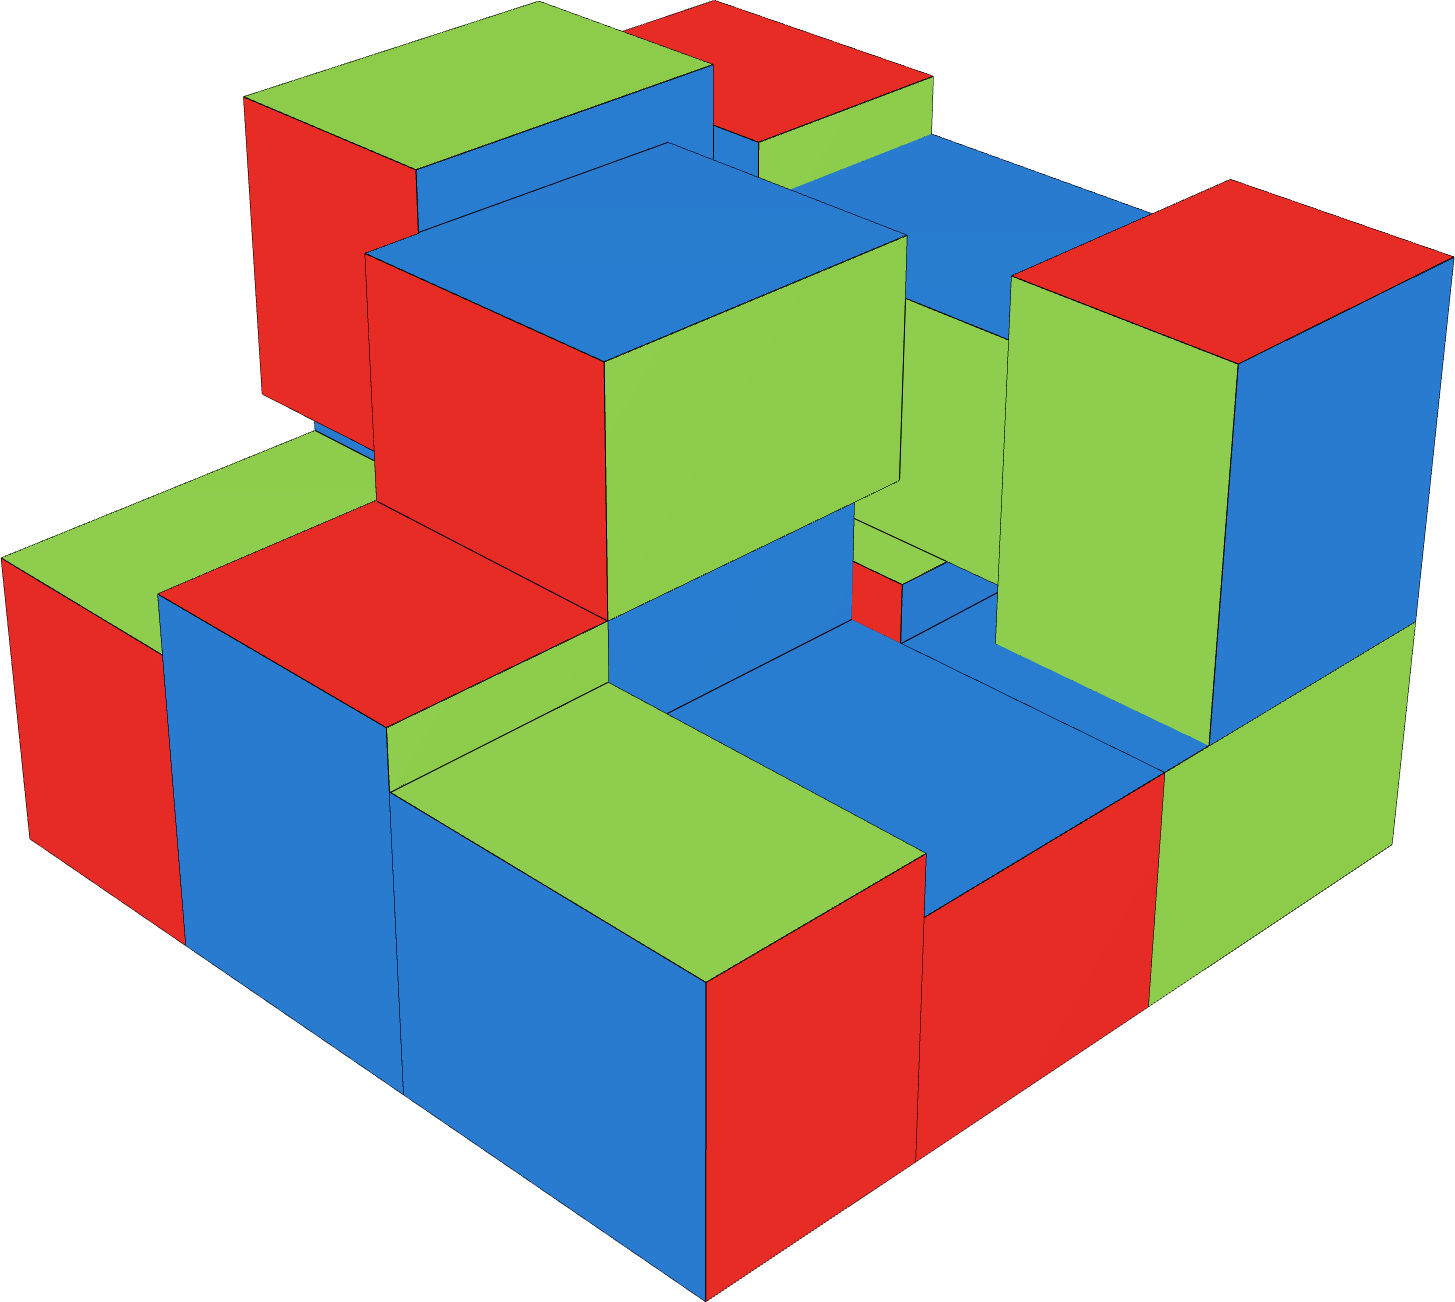
\includegraphics[scale=0.23]{graphics/3d-cube-sharp-corner.png}
        \caption{Sharp corner in three dimensions.}
        \label{fig:3d-sharp-corner-cube}
    \end{subfigure}
    \caption{Examples of sharp corners. Observe that the three-dimensional sharp corner can not be detected by looking at the squares. Thus, while sharp corners of higher dimensions are theoretically possible, they are not easily visualized.}
    \label{fig:3d-sharp-corners}
\end{figure}
\end{remark}

\noindent The next result shows that the No neighbour overlap criterion \labelcref{criterion:no-neighbour-overlap-criterion} is satisfied by any Hoffman packing of a dimension tuple satisfying Hoffman's inequality.

\begin{proposition}\label[proposition]{prop:hoffman-packing-satisfies-nnoc}
Suppose $P\colon G_n \to S_n$ is a Hoffman packing of a dimension tuple $d$ satisfying Hoffman's inequality. Then $P$ satisfies the No neighbour overlap criterion \labelcref{criterion:no-neighbour-overlap-criterion} for $d$.
\end{proposition}
\begin{proof}
Let $(B, C)$ be the packing of $d$ produced by $P$. Suppose $p$ and $q$ are two neighbouring grid point coordinates in $G_n$ and let
\[
R_p = I_1 \times I_2 \times \dotsb \times I_n \quad \text{and} \quad
R_q = J_1 \times J_2 \times \dotsb \times J_n
\]
be their associated hyperrectangles in $B$. Let $\alpha$ and $\beta$ be the actual grid points corresponding to the coordinates $p$ and $q$, respectively. By Hoffman's grid theorem \labelcref{thm:grid-theorem} each grid point lies inside its respective hyperrectangle, i.e.\ $\alpha \in R_p$ and $\beta \in R_q$. Since $(B, C)$ is a packing $R_p$ and $R_q$ are non-overlapping, so by \cref{lemma:overlap} there exists some $k$ in $\curly{1, 2, \dotsc, n}$ such that $I_k$ does not intersect $J_k$. We must have that $\abs{p_k - q_k} = 1$, because otherwise $p_k = q_k$, whereby $\alpha_k = \beta_k$ and $I_k$ would intersect $J_k$. In the notation of the No neighbour overlap criterion \labelcref{criterion:no-neighbour-overlap-criterion} $I_k = (a(p)_k, b(p)_k)$ and $J_k = (a(q)_k, b(q)_k)$. If $p_k < q_k$, then $\alpha_k < \beta_k$. Then $b(p)_k \leq a(q)_k$ to avoid $I_k$ and $J_k$ intersecting one another. Similarly we conclude for $p_k > q_k$ that $b(q)_k \leq a(p)_k$. Hence, $P$ satisfies the No neighbour overlap criterion \labelcref{criterion:no-neighbour-overlap-criterion} for $d$.
\end{proof}

\noindent Next, we show that the No neighbour overlap criterion \labelcref{criterion:no-neighbour-overlap-criterion} and the Line criterion \labelcref{criterion:line-criterion} are enough to ensure that a pseudo-packing is in fact a packing. We will need the following result.

\begin{lemma}\label[lemma]{lemma:ordering-of-sum-by-terms}
Suppose $d = \paren{x_1, x_2, \dotsc, x_n}$ is a dimension tuple satisfying Hoffman's inequality and suppose $A$ and $B$ are two subsets of $D = \curly{1, 2, \dotsc, n}$. If $\abs{A} < \abs{B}$, then
\[
\sum_{i \in A} x_i < \sum_{i \in B} x_i.
\]
\end{lemma}
\begin{proof}
Suppose not.
Let $C = D \setminus A$. Recall that $d$ is increasing by Hoffman's inequality and note that $\abs{C} = n - \abs{A}$, so $\abs{B} + \abs{C} = \abs{B} + n - \abs{A} \geq n + 1$. Then
\begin{align*}
 x_1 + x_2 + \dotsb + x_n
= \sum_{i \in D} x_i
&= \sum_{i \in A} x_i + \sum_{i \in C} x_i \\
&\geq \sum_{i \in B} x_i + \sum_{i \in C} x_i
\geq (\abs{B} + \abs{C}) x_1
\geq (n + 1) x_1,
\end{align*}
which contradicts $d$ satisfying Hoffman's inequality.
\end{proof}

\noindent Intuitively, the sums consisting of distinct terms from $d$ are ordered by the number of terms in each sum. The situation gets significantly more complicated when two sums consist of the same number of terms, and we will return to this scenario in a moment.

\begin{theorem}\label[theorem]{thm:line-and-neighbour-gives-hoffman-packing}
Suppose $P \colon G_n \to S_n$ and suppose $d$ is a dimension tuple satisfying Hoffman's inequality. If $P$ satisfies the Line criterion \labelcref{criterion:line-criterion} and if $P$ satisfies the No neighbour overlap criterion \labelcref{criterion:no-neighbour-overlap-criterion} for $d$, then $P$ is a Hoffman packing of $d$.
\end{theorem}
\begin{proof}
Let $(B, C)$ be the pseudo-packing of $d$ produced by $P$. We need to show that $(B, C)$ is a packing of $d$. Let $s$ be the sum of $d$. Since $P$ satisfies the Line criterion \labelcref{criterion:line-criterion} the stuffing on each grid line is equal to $s$, i.e.\ all grid lines are completely stuffed. By \cref{prop:under-stuffed-contains-rects}, all hyperrectangles in $B$ are contained in the surrounding hypercube $C$. It only remains to show that the hyperrectangles in $B$ are pairwise non-overlapping.

Let $p$ and $q$ be two grid point coordinates in $G_n$ and let $R_p$ and $R_q$ denote their associated hyperrectangles. Next, consider the value of
\[
\delta = \max_{i = 1}^n \, \abs{p_i - q_i}.
\]
If $\delta = 0$, then $p = q$ and there is nothing to check. If $\delta = 1$, then $p$ and $q$ are neighbours and it follows by the No neighbour overlap criterion \labelcref{criterion:no-neighbour-overlap-criterion} that $R_p$ and $R_q$ are non-overlapping. Lastly, suppose $\delta > 1$. Then there exists some $k$ in $\curly{1, 2, \dotsc, n}$ such that $\abs{p_k - q_k} > 1$. Assume without loss of generality that $p_k < q_k$. Consider the $k$'th intervals $(a(p)_k, b(p)_k)$ and $(a(q)_k, b(q)_k)$ in the Cartesian products of $R_p$ and $R_q$, respectively. We would like to show that these do not intersect one another, which can be done by showing that $b(p)_k \leq a(q)_k$. By the construction of $(B, C)$ as described in \cref{def:hoffman-packing} the right endpoint $b(p)_k$ is a sum of $p_k$ terms from $d$, while the left endpoint $a(q)_k$ is a sum of $q_k - 1$ terms, namely
\[
b(p)_k = \sum_{i = 1}^{p_k} w(L(p, k, i))_k
\quad \text{and} \quad
a(q)_k = \sum_{i = 1}^{q_k - 1} w(L(q, k, i))_k.
\]
Since $P$ satisfies the Line criterion \labelcref{criterion:line-criterion}, each term in the sum for $b(p)_k$ can be identified by a distinct index in $\curly{1, 2, \dotsc, n}$. Denote this index set by $A$ and notice that $\abs{A} = p_k$. Similarly we get an index set for $B$ from the sum for $a(q)_k$ and $\abs{B} = q_k - 1$. Note that $\abs{A} = p_k < q_k - 1 = \abs{B}$, so by \cref{lemma:ordering-of-sum-by-terms} $b(p)_k < a(q)_k$. Then $R_p$ and $R_q$ are non-overlapping by \cref{lemma:overlap}. Thus, every pair of hyperrectangles are non-overlapping, so $(B, C)$ is a packing of $d$ and $P$ is a Hoffman packing of $d$.
\end{proof}

\noindent The above proof relies heavily on the dimension tuple $d$ satisfying Hoffman's inequality, where the technicalities have been buried in \cref{lemma:ordering-of-sum-by-terms}. However, experimental results suggest that we do not need to restrict ourselves to dimension tuples satisfying Hoffman's inequality and we will propose a conjecture in relation to this in \cref{sec:truely-universal-packing}.

\begin{remark}
Loosely speaking, Hoffman's inequality forces sums consisting of distinct terms from the increasing dimension tuple $\paren{x_1, x_2, \dotsc, x_n}$ to be ordered by the number of terms in each sum (\cref{lemma:ordering-of-sum-by-terms}). For $n = 3$ this property is actually guarded by the inequality
\begin{equation}\label{eq:3d-no-float-ineq}
    x_3 < x_1 + x_2,
\end{equation}
which Dean G. Hoffman drew our attention to in recent correspondences \cite{hoffman_private}. Observe that any dimension tuple $\paren{x_1, x_2, x_3}$ satisfying Hoffman's inequality will also satisfy \eqref{eq:3d-no-float-ineq}. However, $d' = \paren{2, 3, 4}$ satisfies \eqref{eq:3d-no-float-ineq}, but not Hoffman's inequality. Hence, the conclusion of \cref{lemma:ordering-of-sum-by-terms} and \cref{thm:line-and-neighbour-gives-hoffman-packing} should also hold for $d'$. We suspect the generalization of \eqref{eq:3d-no-float-ineq} to higher dimensions to be
\[
\sum_{i = \ceil*{n/2}+1}^{n} x_i < \sum_{i = 1}^{\ceil*{n/2}} x_i,
\]
and we mention this generalized inequality for future studies, because we suspect it to be a more precise requirement for a packing produced by a Hoffman packing to be rigid, i.e.\ without any ``loose bricks''.
\end{remark}

\subsection{Promoting a Hoffman packing to a universal packing}
By \cref{thm:line-and-neighbour-gives-hoffman-packing} we can guarantee that a map $P\colon G_n \to S_n$ is a universal packing by making sure that it satisfies the Line criterion \labelcref{criterion:line-criterion} and that it satisfies the No neighbour overlap criterion \labelcref{criterion:no-neighbour-overlap-criterion} for any choice of dimension tuple satisfying Hoffman's inequality. This is a lot of dimension tuples to examine and gives rise to the following definition.

\begin{definition}[Representative dimension tuple set]\label[definition]{def:representative-dimension-tuple-set}\index{Dimension tuple!representative set (RDTS)}
Suppose $T$ is a set of increasing dimension tuples. Then $T$ is a \textit{representative dimension tuple set} (RDTS)\index{RDTS|see{Dimension tuple}} if it has the following property: Suppose $P\colon G_n \to S_n$ satisfies the Line criterion \labelcref{criterion:line-criterion} and satisfies the No neighbour overlap criterion \labelcref{criterion:no-neighbour-overlap-criterion} for all dimension tuples in $T$, then $P$ satisfies the No neighbour overlap criterion \labelcref{criterion:no-neighbour-overlap-criterion} for \textit{any} increasing dimension tuple.
\end{definition}

\noindent We can restrict ourselves to maps satisfying the Line criterion \labelcref{criterion:line-criterion}, since it is a requirement for being a universal packing by \cref{prop:universal-packing-has-unique-lines}. Observe that the set of all increasing dimension tuples constitute a RDTS. However, it turns out that far fewer dimension tuples are required to constitute a RDTS. This greatly simplifies the practical search for universal packings, since it enables us to search for universal packings using just a few specific dimension tuples.

Suppose $P\colon G_n \to S_n$ is a map satisfying the Line criterion \labelcref{criterion:line-criterion}. If $P$ satisfies the No neighbour overlap criterion \labelcref{criterion:no-neighbour-overlap-criterion} for all dimension tuples in a RDTS, then it will in fact be a universal packing by \cref{thm:line-and-neighbour-gives-hoffman-packing}. When constructing a RDTS $T$ the strategy will be to include just enough dimension tuples to force $P$ to satisfy the No neighbour overlap criterion \labelcref{criterion:no-neighbour-overlap-criterion} for any choice of increasing dimension tuple as long as $P$ satisfies this criterion for the dimension tuples in $T$.

Suppose $d = \paren{x_1, x_2, \dotsc, x_n}$ is an increasing dimension tuple and let us examine the No neighbour overlap criterion \labelcref{criterion:no-neighbour-overlap-criterion} in more depth. For each pair of neighboring grid point coordinates $p$ and $q$ in $G_n$ the No neighbour overlap criterion \labelcref{criterion:no-neighbour-overlap-criterion} considers a number of inequalities, namely one for each entry where $p$ and $q$ differ. We will refer to such a composition of inequalities as an \textit{overlap comparison}\index{Overlap comparison} and to each of the inequalities as an \textit{overlap inequality}. Consider an overlap inequality from the overlap comparisons of $p$ and $q$. Notice that it has the same number of terms $t$ from $d$ on each side of the inequality sign and that $0 < t < n$. We will refer to the positive integer $t$ as the \textit{arity} of the overlap inequality. Consider the terms on one side. Since $P$ satisfies the Line criterion \labelcref{criterion:line-criterion}, then each term $x_i$ on this side is identified by a unique $i$ in $\curly{1, 2, \dotsc, n}$. Hence, we can identify an overlap inequality in the following way.

\begin{definition}[Overlap inequality]\label[definition]{def:overlap-inequality}\index{Overlap inequality}
Suppose $A$ and $B$ are two non-empty proper subsets of $\curly{1, 2, \dotsc, n}$ with the same cardinality $\abs{A} = \abs{B} = t$. Then $(A, B)$ is an $n$-dimensional \textit{overlap inequality} with \textit{arity}\index{Overlap inequality!arity of} $t$.
\end{definition}

\noindent We say that the dimension tuple $d$ \textit{satisfies}\index{Overlap inequality!satisfied by dimension tuple}\index{Dimension tuple!satisfying overlap inequality} the overlap inequality if
\[
\sum_{i \in A} x_i \leq \sum_{i \in B} x_i.
\]
Be aware that for the sake of readability, we might sometimes write an overlap inequality as above, even if each $x_i$ have not been defined.

Some overlap inequalities are satisfied for any choice of increasing dimension tuple. Suppose $(A, B)$ is an $n$-dimensional overlap inequality with arity $t$. Let $(\alpha_i)_{i=1}^t$ and $(\beta_i)_{i=1}^t$ be the strictly increasing sequences of element in $A$ and $B$, respectively. If $\alpha_i \leq \beta_i$ for all $i = 1, 2, \dotsc, t$, then the overlap inequality is satisfied by any increasing dimension tuple. We will refer to such an overlap inequality as \textit{trivial}\index{Overlap inequality!trivial}. It is convenient to introduce the following equivalence relation between $n$-dimensional increasing dimension tuples. Suppose $d_1 = \paren{x_1, x_2, \dotsc, x_n}$ and $d_2 = \paren{y_1, y_2, \dotsc, y_n}$ are two increasing dimension tuples. We define these dimension tuples to be equivalent if they satisfy the same overlap inequalities, that is for any non-empty proper subsets $A$ and $B$ of $\curly{1, 2, \dotsc, n}$ with $\abs{A} = \abs{B}$, then
\[
\sum_{i \in A} x_i \leq \sum_{i \in B} x_i
\iff
\sum_{i \in A} y_i \leq \sum_{i \in B} y_i.
\]
We denote the equivalence class of $d_1$ by $[d_1]$. Then we can establish a well-defined partial ordering on the equivalence classes, where $[d_1] \leq [d_2]$ if any overlap inequality satisfied by $d_1$ is also satisfied by $d_2$, that is
\[
\sum_{i \in A} x_i \leq \sum_{i \in B} x_i
\implies
\sum_{i \in A} y_i \leq \sum_{i \in B} y_i.
\]
Notice that the equivalence class $[\paren{x_1, x_2, \dotsc, x_n}]$ where $x_1 = x_2 = \dotsb = x_n$ containing the dimension tuple of any hypercube is the greatest element with respect to this ordering, since it satisfies all overlap inequalities. The next result shows how this partial ordering enables us to propagate information about the No neighbour overlap criterion \labelcref{criterion:no-neighbour-overlap-criterion}.

\begin{proposition}\label[proposition]{prop:propagate-nnoc}
Suppose $d_1$ and $d_2$ are two increasing dimension tuples with $[d_1] \leq [d_2]$. If $P\colon G_n \to S_n$ satisfies the Line criterion \labelcref{criterion:line-criterion} and satisfies the No neighbour overlap criterion \labelcref{criterion:no-neighbour-overlap-criterion} for $d_1$, then it does so for $d_2$ as well.
\end{proposition}
\begin{proof}
Since $P$ satisfies the Line criterion \labelcref{criterion:line-criterion} all overlap comparisons consist of inequalities which can be identified as in \cref{def:overlap-inequality}. Since $[d_1] \leq [d_2]$ the overlap inequalities satisfied by $d_1$ are satisfied by $d_2$ as well. Then $P$ satisfies the No neighbour overlap criterion \labelcref{criterion:no-neighbour-overlap-criterion} for $d_2$.
\end{proof}

\noindent The construction of these equivalence classes enables us to show the following result.

\begin{proposition}
The number of equivalence classes of increasing dimension tuples is finite.
\end{proposition}
\begin{proof}
Let us begin by establishing an upper bound on the number of different overlap inequalities. First, we count the number of overlap inequalities with a certain arity. Pick some arity $t$ and note that $0 < t < n$. The number of subsets of $\curly{1, 2, \dotsc, n}$ with $t$ elements is $\binom{n}{t}$, so the number of overlap inequalities with arity $t$ is $\binom{n}{t}^2$. Hence the total number of overlap inequalities is
\[
k = \sum_{i = 1}^{n - 1} \binom{n}{i}^n.
\]
When determining which equivalence class an increasing dimension tuple belongs to it depends on which overlap inequalities are satisfied and which are not. Hence, the number of equivalence classes is no greater than $2^k$.
\end{proof}

\noindent This information implies that there exists a finite RDTS in any dimension $n$, since we can construct such a set by picking a representative from each of the finitely many equivalence classes. We can actually show that any equivalence class has a representative satisfying Hoffman's inequality. Having a RDTS consisting of dimension tuples all satisfying Hoffman's inequality simplifies the search for a universal packing due to \cref{prop:hoffman-packing-satisfies-nnoc}.

\begin{proposition}\label[proposition]{prop:exists-representative-satisfying-hoffman-ineq}
Suppose $d$ is an increasing dimension tuple. Then there exists a dimension tuple $d'$ satisfying Hoffman's inequality and such that $[d] = [d']$.
\end{proposition}
\begin{proof}
Let $d = \paren{x_1, x_2, \dotsc, x_n}$ and let $c = \sum_{i = 1}^n \paren{x_i - x_1}$ and note that $c \geq 0$. Let $d' = \paren{y_1, y_2, \dotsc, y_n}$ where $y_i = x_i + c$ for all $i = 1, 2, \dotsc, n$. Note that for any overlap inequality $(A, B)$
\[
\sum_{i \in A} x_i \leq \sum_{i \in B} x_i \iff
\sum_{i \in A} \paren{x_i + c} \leq \sum_{i \in B} \paren{x_i + c} \iff
\sum_{i \in A} y_i \leq \sum_{i \in B} y_i,
\]
since $\abs{A} = \abs{B}$, whereby $[d] = [d']$. Next, we see that
\[
\sum_{i = 1}^n \paren{y_i - y_1} =
\sum_{i = 1}^n \paren{x_i - x_1} =
c < x_1 + c = y_1,
\]
and it follows that $d'$ satisfies Hoffman's inequality as desired.
\end{proof}

\noindent In addition, we can do better in order to reduce the number of dimension tuples necessary to constitute a RDTS.

\begin{proposition}\label[proposition]{prop:minimal-rdts}
Suppose $T$ is a set of increasing dimension tuples such that $T$ contains a representative from each minimal equivalence class. Then $T$ is a RDTS.
\end{proposition}
\begin{proof}
Suppose $P\colon G_n \to S_n$ satisfies the Line criterion \labelcref{criterion:line-criterion} and satisfies the No neighbour overlap criterion \labelcref{criterion:no-neighbour-overlap-criterion} for all dimension tuples in $T$. Suppose $d$ is an increasing dimension tuple. By the construction of $T$ there must be some dimension tuple $d'$ in $T$ such that $[d'] \leq [d]$. Since $P$ satisfies the No neighbour overlap criterion \labelcref{criterion:no-neighbour-overlap-criterion} for $d'$, then by \cref{prop:propagate-nnoc} it does so for $d$ as well. Hence, $T$ is a RDTS.
\end{proof}

\noindent Thus, if we can show that some equivalence class is in fact the least element, then the set consisting of just one of the dimension tuples from this equivalence class will constitute a RDTS. Next, we show a result which simplifies determining a small RDTS, and give an example of using it in the two-dimensional case.

\begin{proposition}\label[proposition]{prop:arity-1-trivial}
Suppose $d$ is an increasing dimension tuple with distinct elements. Then any overlap inequality with arity 1 satisfied by $d$ is trivial.
\end{proposition}
\begin{proof}
Let $d = \paren{x_1, x_2, \dotsc, x_n}$ and observe that it must be strictly increasing. Suppose $(A, B)$ is an overlap inequality with arity 1, i.e.\ $A$ and $B$ are non-empty proper subsets of $\curly{1, 2, \dotsc, n}$ with $\abs{A} = \abs{B} = 1$. Then we can write $A = \curly{i}$ and $B = \curly{j}$ for some $i$ and $j$ in $\curly{1, 2, \dotsc, n}$. If $i \leq j$, then the overlap inequality is trivial. Suppose not, i.e. $i > j$. Then $x_i \leq x_j$, which contradicts $d$ being strictly increasing.
\end{proof}

\begin{example}[RDTS for $n = 2$]
In this case all overlap inequalities have arity $1$. For an increasing dimension tuple $(x_1, x_2)$ there are four overlap inequalities,
\[
x_1 \leq x_1, \quad x_1 \leq x_2, \quad x_2 \leq x_1 \quad \text{and} \quad x_2 \leq x_2.
\]
Three of these are trivial, while $x_2 \leq x_1$---strictly speaking identified by the tuple $(\curly{2}, \curly{1})$---is the only non-trivial overlap inequality. Observe that $d = \paren{2, 3}$ satisfies Hoffman's inequality and contains distinct elements. Then $d$ satisfies only trivial overlap inequalities by \cref{prop:arity-1-trivial}. Hence $[d]$ is the least element, so by \cref{prop:minimal-rdts}
\[
T = \curly{\paren{2, 3}}
\]
is a RDTS for $n = 2$.
\end{example}

\noindent Before considering the three-dimensional case, we will show that an overlap inequality with sufficiently high arity is actually an overlap inequality with a lower arity in disguise. Intuitively, it has so many terms on each side of the inequality sign that some identical terms must occur on both sides. Subtracting these terms from both sides yields an overlap inequality with lower arity, which is satisfied precisely when the original overlap inequality is satisfied.

\begin{lemma}\label[lemma]{lemma:arity-minus-common-terms}
Suppose $(A, B)$ is a non-trivial $n$-dimensional overlap inequality with arity $s$. Then there exists an overlap inequality $(A', B')$ with arity $s - \abs{A \cap B}$ which is satisfied precisely when $(A, B)$ is satisfied.
\end{lemma}
\begin{proof}
Note that $A \neq B$, since the overlap inequality is non-trivial. Let $C = A \cap B$, $A' = A \setminus C$ and $B' = B \setminus C$. Then
\[
\sum_{i \in A} x_i \leq \sum_{i \in B} x_i
\iff
\sum_{i \in A'} x_i + \sum_{i \in C} x_i \leq \sum_{i \in B'} x_i + \sum_{i \in C} x_i
\iff
\sum_{i \in A'} x_i \leq \sum_{i \in B'} x_i
\]
for any increasing dimension tuple $d = \paren{x_1, x_2, \dotsc, x_n}$. Finally, note that $\paren{A', B'}$ has arity $t = s - \abs{A \cap B}$ and that $0 < t$, since $\abs{A \cap B} < s$.
\end{proof}

\begin{proposition}\label[proposition]{prop:arity-reduction}
Suppose $(A, B)$ is an $n$-dimensional overlap inequality. Then there exists an overlap inequality $(A', B')$ with arity $t$ such that $0 < t \leq n/2$ and which is satisfied precisely when $(A, B)$ is satisfied.
\end{proposition}
\begin{proof}
If $n = 1$ there are no overlap inequalities, so suppose $n \geq 2$. Let $s$ be the arity of $(A, B)$, that is $s = \abs{A} = \abs{B}$. If $s \leq n/2$ we are done by choosing $(A', B')$ to be $(A, B)$. Suppose $s > n/2$. If $A = B$, then the overlap inequality is trivial and we can simply choose $(A', B') = (\curly{1}, \curly{1})$. Otherwise by \cref{lemma:arity-minus-common-terms} there exists an overlap inequality $(A', B')$ with arity $t = s - \abs{A \cap B}$ which is satisfied precisely when $(A, B)$ is satisfied. We claim that $t \leq n/2$. Otherwise $n/2 < t$ and
\[
n < 2t = 2s - 2\abs{A \cap B}
= \abs{A} + \abs{B} - 2\abs{A \cap B}
= \abs{A \cup B} - \abs{A \cap B}
\leq \abs{A \cup B},
\]
which is impossible as $A$ and $B$ are subsets of $\curly{1, 2, \dotsc, n}$ with only $n$ elements.
\end{proof}

\begin{example}[RDTS for $n = 3$]\label[example]{ex:3d-rdts}
In this case all overlap inequalities have arity $1$ or $2$. Observe that $d = \paren{4, 5, 6}$ satisfies Hoffman's inequality and contains distinct elements. Of the overlap inequalities with arity $1$, then $d$ satisfies only the trivial ones by \cref{prop:arity-1-trivial}. We will show that the same is the case for overlap inequalities with arity $2$. Suppose $(A, B)$ is an overlap inequality with arity $2$ which is satisfied by $d$. Then by \cref{prop:arity-reduction} there exists an overlap inequality $(A', B')$ with arity $1$ which is also satisfied by $d$. But then $(A, B)$ is trivial itself. Hence $d$ satisfies only trivial overlap inequalities, so $[d]$ is the least element and by \cref{prop:minimal-rdts}
\[
T = \curly{\paren{4, 5, 6}}
\]
is a RDTS for $n = 3$. Hence, we can use this specific dimension tuple when searching for three-dimensional universal packings.
\end{example}
